\chapter{Burglar's Night Out}

\section{Problem Statement}

A burglar has come to your neighborhood at night. Your neighborhood has many houses arranged in a linear fashion and each house has some amount of money. The burglar wishes to take as much money as possible. However, he cannot rob two consecutive houses otherwise the security bell will ring and he will get caught.

\begin{figure}[H]
    \centering
    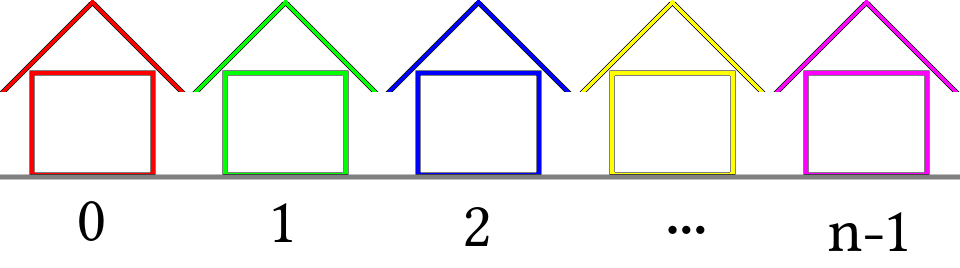
\includegraphics[width=\textwidth]{images/blurglars_night_out/houses.png}
\end{figure}

\section{Basic Definitions}

\newcommand{\binarySet}{\ensuremath{\mathbb{B}}}
\renewcommand{\cost}[2]{\ensuremath{\apply{\sigma_{#2}}{#1}}}

\begin{defn}[Binary Sequence and Real Sequence]
    A \textbf{Binary Sequence} is a sequence of values of the binary set $\binarySet = \Set{True, False}$.
    A \textbf{Real Sequence} is a sequence of values of the real set $\R$.
\end{defn}

\begin{defn}[Cost of a Sequence]
    Given a Binary Sequence $b$ and a real sequence $r$, both with the same length, the \textbf{Cost $\cost{b}{r}$ of the Sequence $b$} with values $r$ is given by:
    \begin{equation}
        \cost{b}{r} = \Sum{i \in \SetOf{i \in \range{n}}{b[i] = True}}{}{r[i]}
    \end{equation}
\end{defn}

\begin{defn}[True Alternate Binary Sequence]
    A Binary Sequence $b$ is called \textbf{True Alternate Binary Sequence} or simply \textbf{True Alternate} if there are no two consecutive values in which both are $True$. In other words:
    \begin{align}
        & \forall i \in \range{n} \nexists j \in \range{n} \left(
            j = i + 1
            \land
            i = True
            \land
            j = True
        \right)
        & \equiv \\\nonumber
        &
        \forall i \Big(
            \left(i \in \range{n} \land i = True\right)
            \rightarrow
            \nexists j \left(
                j \in \range{n}
                \land
                j = i + 1
                \land
                j = True
            \right)
        \Big) &
    \end{align}
\end{defn}

\section{Problem Definition}

\begin{enumerate}
    \item Input:
    \begin{enumerate}
        \item the number of houses: a natural number $n \in \N$;
        \item the cost sequence: a Real Sequence $r$ of length $n$;
    \end{enumerate}
    \item Output: a True Alternate Binary Sequence $b$ of length $n$;
    \item Goal: Maximize the cost of the sequence $\cost{b}{r}$;
\end{enumerate}

\section{Naive Algorithm}

\begin{algorithm}[H]
    \caption{Naive}
    \label{burglar's-night-out:algorithm:naive}
    \begin{algorithmic}[1]
        \Require{$n \in \N, r \in \R^n$}
        \State{$S \gets \mbox{generate\_all\_binary\_sequences}(n)$}
        \State{$S' \gets \mbox{filter\_true\_alternate\_sequences}(S)$}
        \State{$s^* \gets \ArgMax{s \in S'}{\cost{s}{r}}$}
        \State{\textbf{return} $s^*$}
    \end{algorithmic}
\end{algorithm}

\section{Dynamic Programming}

\subsection{Initialization}

Initialize the problem with two optimal solutions for the problem of size 1:

\begin{enumerate}
    \item $\tuple{true}$  (i.e. the optimal solution which uses the value $r[0]$);
    \item $\tuple{false}$ (i.e. the optimal solution which does not use the value $r[0]$);
\end{enumerate}

\subsection{Optimal Subproblem Structure}

Suppose one has two optimal solutions for the subproblem of size $i < n$:

\begin{enumerate}
    \item the optimal solution which uses the value $r[i]$ (i.e. $b[i] = True$);
    \item the optimal solution which does not use the value $r[i]$ (i.e. $b[i] = False$);
\end{enumerate}

The solution for the subproblem of size $i+1$ is the best one among the following:

\begin{enumerate}
    \item\label{burglar's-night-out:dp:case:use-i+1} do not use $r[i]$; use $r[i+1]$;
    \item\label{burglar's-night-out:dp:case:use-i} use $r[i]$, do not use $r[i+1]$;
    \item\label{burglar's-night-out:dp:case:use-none} do not use $r[i]$; do not use $r[i+1]$\footnote{This case does not have to be here if the cost sequence $r$ has only non-negative values. But since one allowed negative costs, this case has to be considered.};
\end{enumerate}

\ref{burglar's-night-out:dp:case:use-i+1} is the best solution which uses $r[i+1]$. The best among \ref{burglar's-night-out:dp:case:use-i} and \ref{burglar's-night-out:dp:case:use-none} is the best solution which does not use $r[i+1]$.

Finally, the best solution for the problem of size $n$ (the original problem) is the best between the two: the one which uses $r[n-1]$ and the one which doesn't use it.

\subsection{Algorithm Description}

\begin{algorithm}
    \begin{lstlisting}
        object SubproblemSolutions {
          lastIncluded: BinarySequence
          lastExcluded: BinarySequence
        }
    \end{lstlisting}
    \caption{data structure $SubproblemSolutions$.}
\end{algorithm}

\begin{algorithm}[H]
    \caption{Dynamic Programming}
    \label{burglar's-night-out:algorithm:dynamic-programming}
    \begin{algorithmic}[1]
        \Require{$n \in \N, r \in \R^n$}
        \State{// Initialization}
        \State{$S \gets vector<SubproblemSolutions>$}
        \State{$s \gets SubproblemSolutions(lastIncluded = \tuple{true}, lastExcluded = \tuple{false})$}
        \State{$S.append(s)$}
        \State{// Rescursive solver}
        \For{$ i \in \Set{1, \dots, n-1}$}
            \State{// last included}
            \State{$lastIncluded \gets S[i-1].lastExcluded$}
            \State{$lastIncluded.append(True)$}
            \State{// last excluded}
            \State{$lastExcluded \gets \ArgMax{s \in S[i-1]}{\cost{s}{r}}$}
            \State{$lastExcluded.append(False)$}
            \State{// next entry}
            \State{$S.append(SubproblemSolutions(lastIncluded, lastExcluded))$}
        \EndFor{}
        \State{// Optimal solution of the original problem}
        \State{$s^* \gets \ArgMax{s \in S[n-1]}{\cost{s}{r}}$}
        \State{\textbf{return} $s^*$}
    \end{algorithmic}
\end{algorithm}
